\documentclass[frenchb, paper=a4, fontsize=11pt]{scrartcl}

\usepackage[utf8x]{inputenc}
\usepackage[T1]{fontenc}
\usepackage{lmodern}

\usepackage{url}

% Color
% cfr http://en.wikibooks.org/wiki/LaTeX/Colors
\usepackage{color}
\usepackage[usenames,dvipsnames,svgnames,table]{xcolor}
\definecolor{dkgreen}{rgb}{0.25,0.7,0.35}
\definecolor{dkred}{rgb}{0.7,0,0}

\newcommand{\matlab}{\textsc{Matlab}}

% Math symbols
\usepackage{amsmath}
\usepackage{amssymb}
\usepackage{amsthm}

\newcommand\eqdef{\triangleq}

\DeclareMathOperator{\newdiff}{d} % use \dif instead
\newcommand{\dif}{\newdiff\!}
\newcommand{\fpart}[2]{\frac{\partial #1}{\partial #2}}
\newcommand{\ffpart}[2]{\frac{\partial^2 #1}{\partial #2^2}}
\newcommand{\fdpart}[3]{\frac{\partial^2 #1}{\partial #2\partial #3}}
\newcommand{\fdif}[2]{\frac{\dif #1}{\dif #2}}
\newcommand{\ffdif}[2]{\frac{\dif^2 #1}{\dif #2^2}}
\newcommand{\constant}{\ensuremath{\mathrm{cst}}}

\usepackage{siunitx}

\usepackage{tikz}

\usepackage{lmodern}
%\usepackage[protrusion=true,expansion=true]{microtype}
\usepackage{xspace}

\usepackage{babel}

\KOMAoptions{DIV=last}

\usepackage{hyperref}
\usepackage{todonotes}
\usepackage[makeroom]{cancel}

\newcommand*\eq[1]{\overline{#1}} 				% equilibre


%%% Equation and float numbering
\numberwithin{equation}{section}					% Equationnumbering: section.eq#
\numberwithin{figure}{section}					% Figurenumbering: section.fig#
\numberwithin{table}{section}						% Tablenumbering: section.tab#

%%% Maketitle metadata
\newcommand{\horrule}[1]{\rule{\linewidth}{#1}} 	% Horizontal rule

\title{
		%\vspace{-1in} 	
		\usefont{OT1}{bch}{b}{n}
		\normalfont \normalsize \textsc{Ecole polytechnique de Louvain} \\ [25pt]
		\horrule{0.5pt} \\[0.4cm]
		\large LINMA1510 - Automatique linéaire\\
		\huge Laboratoire 1 - Contrôle du niveau d'eau dans un réservoir \\
		\horrule{1.5pt} \\[0.5cm]
}
\author{
		\normalfont
		\textsc{Groupe 62}\\
      	Antoine Paris\hspace{0.6cm} Philippe Verbist \\	
       	\normalsize
        \today
}
\date{}

\begin{document}
\maketitle

Les notations utilisées dans ce document sont définies dans la section 3.1
de l'énoncé.

\section{Modèle du système}
Le modèle utilisé vient des équations de \textsc{Bernoulli} de la
conservation d'énergie. Il utilise les deux équations suivantes
\begin{itemize}
	\item équation de continuité
	\begin{equation}
		\frac{dh_3}{dt} = \frac{1}{S_R}q_{P3} - \frac{1}{S_R}(q_{F30}+q_{S30}).
		\label{eq:contnuity}
	\end{equation}
	\item loi de \textsc{Toricelli}
	\begin{align}
		q_{F30} &= S_{F30} \sqrt{2gh_3} \label{eq:toricelliF}, \\
		q_{S30} &= S_{S30} \sqrt{2gh_3} \label{eq:toricelliS}.
	\end{align}
\end{itemize}
Ce modèle est donc clairement \textbf{non-linéaire}.
En outre, les constantes suivantes sont données
\begin{align}
	S_R	&= \SI{43}{\cm\squared}, \\
	g 	&= \SI{981}{\cm\per\second\squared}.
\end{align}

\section{Point d'équilibre du système}
Durant cette expérience, la valve $V_{F30}$ --- qui représente
une perturbation apportée au système --- est fermée. Cela
implique $S_{F30} = q_{F30} = 0$. On peut donc réecrire le modèle à l'aide
d'une seule équation
\begin{equation}
	\frac{dh_3}{dt} = \frac{1}{S_R}q_{P3} - \frac{1}{S_R}(S_{S30} \sqrt{2gh_3}).
	\label{eq:syst-model}
\end{equation}

Afin de linéariser le système modélisé par l'équation \ref{eq:syst-model},
il faut avant trouver un point d'équilibre.

\begin{figure}[!ht]
	\centering
	\includegraphics[width=1.0\textwidth]{img/exp1_ol.eps}
	\caption{Réponse du système en boucle ouverte, avec $\eq{q}_{P3} = u_0 =
	\SI{30}{\milli\liter\per\second}$.}
	\label{fig:exp1_ol}
\end{figure}

Pour trouver ce point d'équilibre, la valeur de $q_{P3}$ a été imposée
(arbitrairement) à $\eq{q}_{P3} = u_0 = \SI{30}{\milli\liter\per\second}$. On
mesure ensuite la hauteur $\eq{h}_3$ atteinte
par le système à l'équilibre. Sur la figure \ref{fig:exp1_ol}, on
mesure une valeur de
\begin{equation}
	\eq{h}_3 = \SI{10.1}{\cm}.
\end{equation}

La valeur de $S_{S30}$ reste encore inconnue dans l'équation
\ref{eq:syst-model}. On peut cependant la déterminer grâce
à l'état d'équilibre du système. Par définition de
l'équilibre, on a $\fdif{h_3}{t} = 0$. On connait
également les valeurs de $\eq{q}_{P3}$ et $\eq{h}_3$.
En remplaçant tout cela dans l'équation \ref{eq:syst-model}, on
obtient successivement
\begin{align}
	0 			& = \frac{1}{S_R}\eq{q}_{P3} - \frac{1}{S_R}(S_{S30}\sqrt{2g\eq{h}_3}) \\
	\eq{q}_{P3}	& = S_{S30}\sqrt{2g\eq{h}_3} \\
	S_{S30} 		& = \frac{\eq{q}_{P3}}{ \sqrt{2g\eq{h}_3}} = \SI{0.21}{cm^2}.
\end{align}

\paragraph{Note} pour arriver à des \SI{}{\cm\squared}, on doit utiliser le fait
que \SI{1}{\milli\liter} = \SI{1}{cm^3} pour l'eau.

\section{Linéarisation}
Cette section utilise les notations et la méthode développée dans le document
\og Notice générale pour les laboratoires et les exercices \fg{}. 

\subsection{Modèle linéarisé}
L'état, l'entrée et la perturbation du système sont respectivement
donnés par
\begin{align}
	x &= h_3, 	\\
	u &= q_{P3},	\\
	v &= S_{F30}.
\end{align}
Ces 3 grandeurs sont reliées entre elles par les deux équations
suivantes
\begin{align}
	\frac{dx}{dt} 	&= f(x,u,v) = \frac{1}{S_R}u - \frac{1}{S_R}(v\sqrt{2gx}
	+ S_{S30}\sqrt{2gx})\\
	y 				&= h(x,u,v) = x
\end{align}
Pour linéariser ce système, on procède aux changements de variables
\begin{align}
	\chi 	&= x - \eq{x} 	= x - 10.1	\\
	\rho 	&= u - \eq{u} 	= u - 30		\\
	\nu		&= v - \eq{v} 	= v			\\
	\phi 	&= y - h(\eq{x})	= y - 30
\end{align}
dans lesquels les valeurs d'équilibre précedemment calculées ont été
introduites.
On peut ensuite réécrire le système sous la forme
\begin{equation}
	\left\{	\begin{array}{ccc}
				\frac{d\chi}{dt} &=& A\chi + B\rho \\
				\phi &=& C\chi + D\rho
			\end{array}
	\right.
\end{equation}
avec 
\begin{align*}
	A & = \fpart{f}{x}\Big|_{(\eq{x},\eq{u},\eq{v})} =
	-\frac{1}{S_R}(v\frac{g}{\sqrt{2gx}} + S_{S30}\frac{g}{\sqrt{2gx}})
	\Big|_{(\eq{x},\eq{u},\eq{v})} = -\frac{S_{S30}}{S_R}
	\frac{g}{\sqrt{2g\eq{x}}} = \SI{-0.0345}{\per\second}\\
	B &=	\left[\begin{array}{l}
 			\fpart{f}{u}\Big|_{\eq{x}} \\
  			\fpart{f}{v}\Big|_{\eq{x}} \\
		\end{array} \right] 
	= 	\left[\begin{array}{l}
 			\frac{1}{S_R} \\
  			-\frac{\sqrt{2g\eq{x}}}{S_R}
		\end{array} \right]
	=	\left[\begin{array}{l}
			\SI{0.0233}{\per\centi\meter\squared} \\
			\SI{-3.27}{\per\second}
		\end{array} \right] \\
	C &= \fpart{h}{x}\Big|_{\eq{x}} = 1 \\
	D &= \left[\begin{array}{l}
 			\fpart{h}{u}\Big|_{\eq{x}} \\
  			\fpart{h}{v}\Big|_{\eq{x}}
		\end{array} \right] 
	= 	\left[ \begin{array}{l}
			\SI{0}{\centi\meter\per\milli\liter\per\second} \\
			\SI{0}{\per\centi\meter}
		\end{array} \right]
\end{align*}

% TODO : @pverbist95 can you check units above?

\subsection{Fonctions de transfert}
Pour obtenir les fonctions de transfert $G(s) \equiv q_{P3} \to h_3$
et $H(s) \equiv S_{F30} \to h_3$, on utilise le principe de superposition
en annulant successivement $S_{F30}$ pour trouver $G(s)$ et $q_{P3}$ pour
trouver $H(s)$. En notant $B = [B_u B_v]^t$, cela done
\begin{align}
	G(s) &= C(sI-A)^{-1}B_u + D = \frac{B_u}{s-A}	= \frac{0.0233}{s+0.0345} \\
	H(s) &= C(sI-A)^{-1}B_v + D = \frac{B_v}{s-A} = \frac{-3.27}{s+0.0345}
\end{align}

Remarquons que l'on peut calculer la constante de temps du système en boucle
ouverte
\begin{equation}
	\tau_{OL} = -\frac{1}{A} \approx \SI{29}{s}.
\end{equation}
Notons également que cette constante de temps correspond au système linéarisé
autour de $(\eq{h}_3, \eq{q}_{P3})$, elle n'est donc pas observable sur
la figure \ref{fig:exp1_ol}.

\section{Fonctions de transfert en boucle fermée}
Nous considérons maintenant un contrôleur PI tel que représenté
à la figure \ref{fig:closed_loop}. La fonction de transfert du
régulateur est donnée par
\begin{equation}
	C(s) = K_P\left(1+\frac{K_I}{s}\right).
\end{equation}

\begin{figure}[!ht]
	\centering
	\includegraphics[width=\linewidth]{img/closed_loop.png}
	\caption{Diagramme de bloc du système contrôlé par un contrôleur PI.}
	\label{fig:closed_loop}
\end{figure}

On trouve
\begin{align}
	T_r(s) 	& \triangleq \frac{y}{r}\Big|_{v=0} = \frac{C(s)G(s)}{1+C(s)G(s)} \\
			&= \frac{B_uK_P(s+K_I )}{s^2 +(B_uK_P-A)s + B_u K_P K_I}.
\end{align}

De même,
\begin{align}
	T_v(s)	& \triangleq \frac{y}{v}\Big|_{r=0} = \frac{H(s)}{1+C(s)G(s)}\\
			& = \frac{B_v s}{s^2 + (B_u K_P-A)s + B_u K_P K_I}.
\end{align}

\section{Analyse des performances d'un contrôleur sans perturbation}
En utilisant $\left\{K_P,K_I\right\}=\left\{2.5,2\right\}$ comme
paramètres du contrôleur, le système en boucle fermée est très peu
controlable, comme illustré à la figure \ref{fig:test1}.

Les oscillations amorties sont effectivement prédites par la théorie
étant donné que $0 < \zeta < 1$. En revanche, la théorie prévoit un
amortissement plus rapide des oscillations.

\begin{figure}
  \centering
  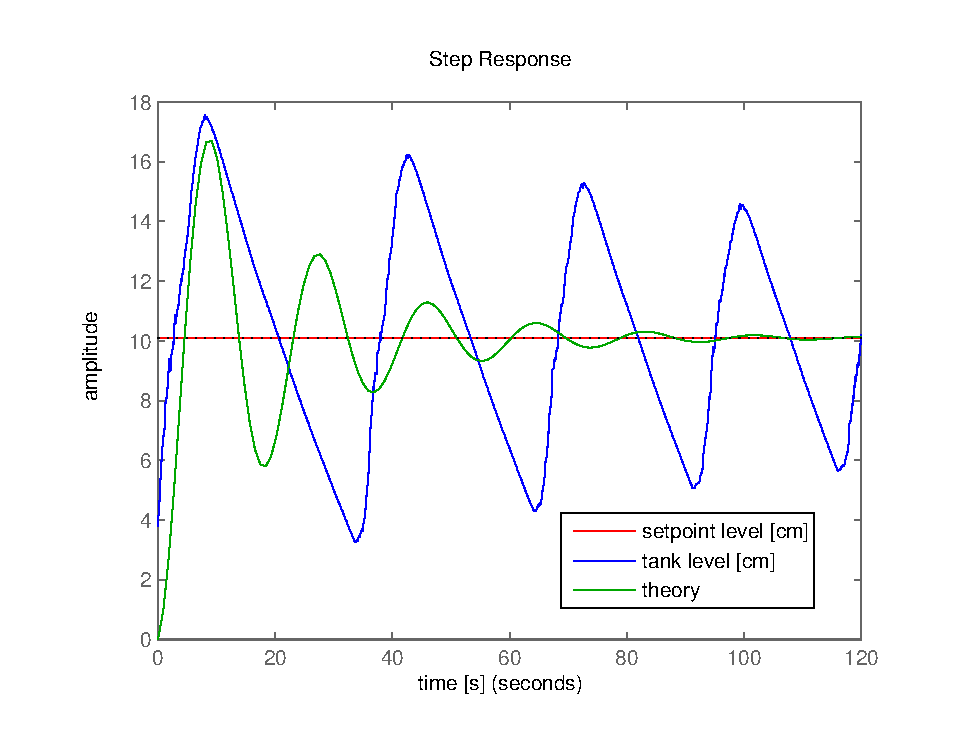
\includegraphics[width=1.0\linewidth]{img/cl-2_5-2-im.eps}
  \captionof{figure}{$\left\{K_P,K_I\right\}=\left\{2.5,2\right\}$.}
  \label{fig:test1}
\end{figure}

\section{Analyse des performances de différents contrôleurs avec une perturbation}
Voir figure \ref{fig:test2}, \ref{fig:test3} et \ref{fig:test4}.

\begin{figure}[!ht]
  \centering
  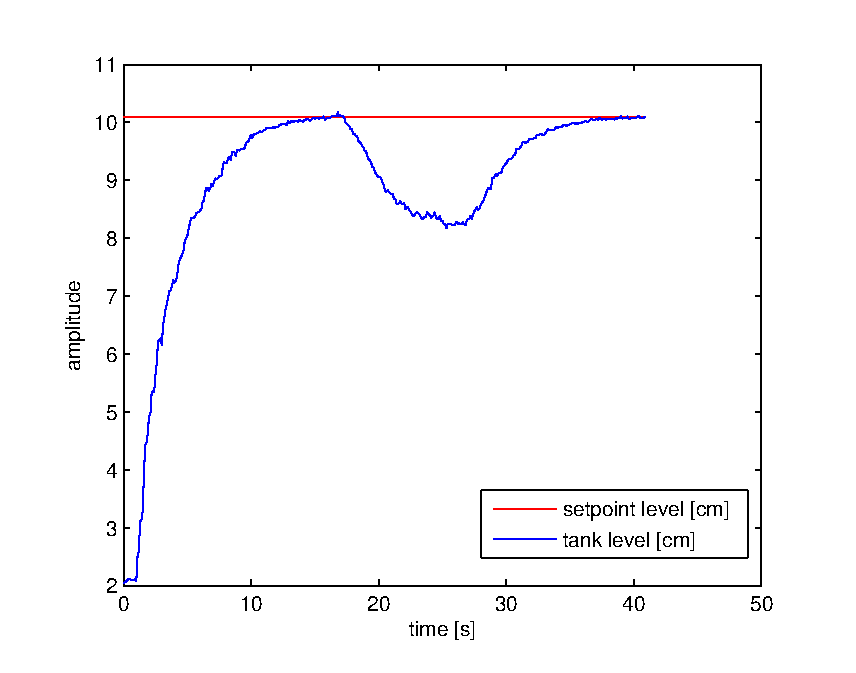
\includegraphics[width=.99\linewidth]{img/cl-10-0.eps}
  \captionof{figure}{$\left\{K_P,K_I\right\}=\left\{10,0\right\}$.}
  \label{fig:test2}
\end{figure}

\begin{figure}[!ht]
\centering
\begin{minipage}{.5\textwidth}
  \centering
  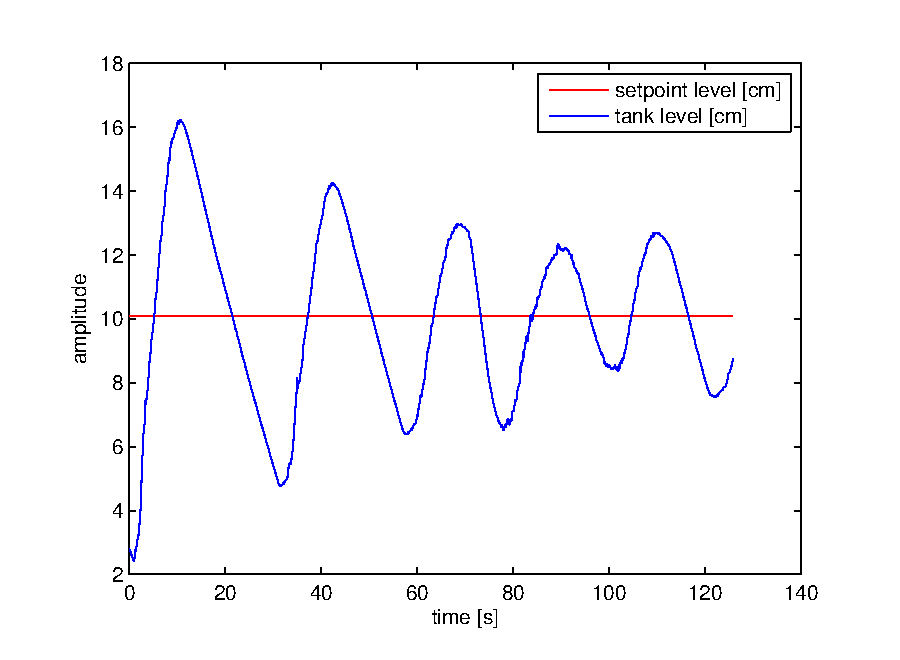
\includegraphics[width=.99\linewidth]{img/cl-3-1.eps}
  \captionof{figure}{$\left\{K_P,K_I\right\}=\left\{3,1\right\}$.}
  \label{fig:test3}
\end{minipage}%
\begin{minipage}{.5\textwidth}
  \centering
  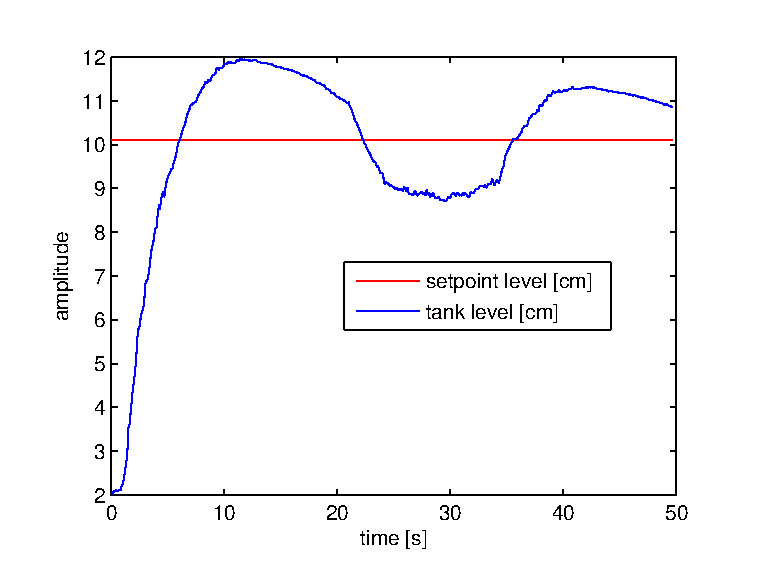
\includegraphics[width=.99\linewidth]{img/cl-10-0_1.eps}
  \captionof{figure}{$\left\{K_P,K_I\right\}=\left\{10,0.1\right\}$.}
  \label{fig:test4}
\end{minipage}
\end{figure}

\section{Calcul des paramètres du PI pour satisfaire certaines spécifications}

\subsection{Sans simplification}
Les spécifications sont:
\begin{itemize}
\item pas d'overshoot ;
\item un temps de réponse trois fois plus petit que le système naturel (non contrôlé).
\end{itemize}
Reprenons le dénominateur de la fonction de transfert $T_r(s)$:
\begin{equation}
	D(s) = s^2 +(B_u K_P -A)s + B_u K_P K_I
\end{equation}
La forme canonique du dénominateur d'un système du deuxième ordre
est donnée par
\begin{equation}
	D_c(s) = s^2 + 2\zeta \omega_n s + \omega_n^2.
\end{equation}
Par identification, on obtient
\begin{align}
	\omega_n 	&= \sqrt{B_u K_P K_I} \label{eq:ns_omegan}\\
	\zeta 		&= \frac{B_u K_P-A}{2\sqrt{B_u K_P K_I}}
\end{align}
Les spécifications nous imposent:
\begin{align}
	\zeta &\ge 1\\
	\tau & = \frac{1}{\omega_n(\zeta - \sqrt{\zeta^2-1})} = \frac{\tau_{OL}}{3}\approx \SI{10}{s} \label{eq:ns_tau}
\end{align}
En imposant $\zeta = 1.5$, et en résolvant les équations \ref{eq:ns_omegan} à \ref{eq:ns_tau},
on trouve
\begin{align}
	K_P &= 18.97\\
	K_I &= 0.0891
\end{align}
La présence d'un zéro dans la fonction de transfert fait apparaitre un overshoot
qu'il n'est pas possible de contrôler de manière canonique. 
La comparaison théorie/résultats se trouve à la figure \ref{fig:final_values_1}.

\begin{figure}[!ht]
	\centering
	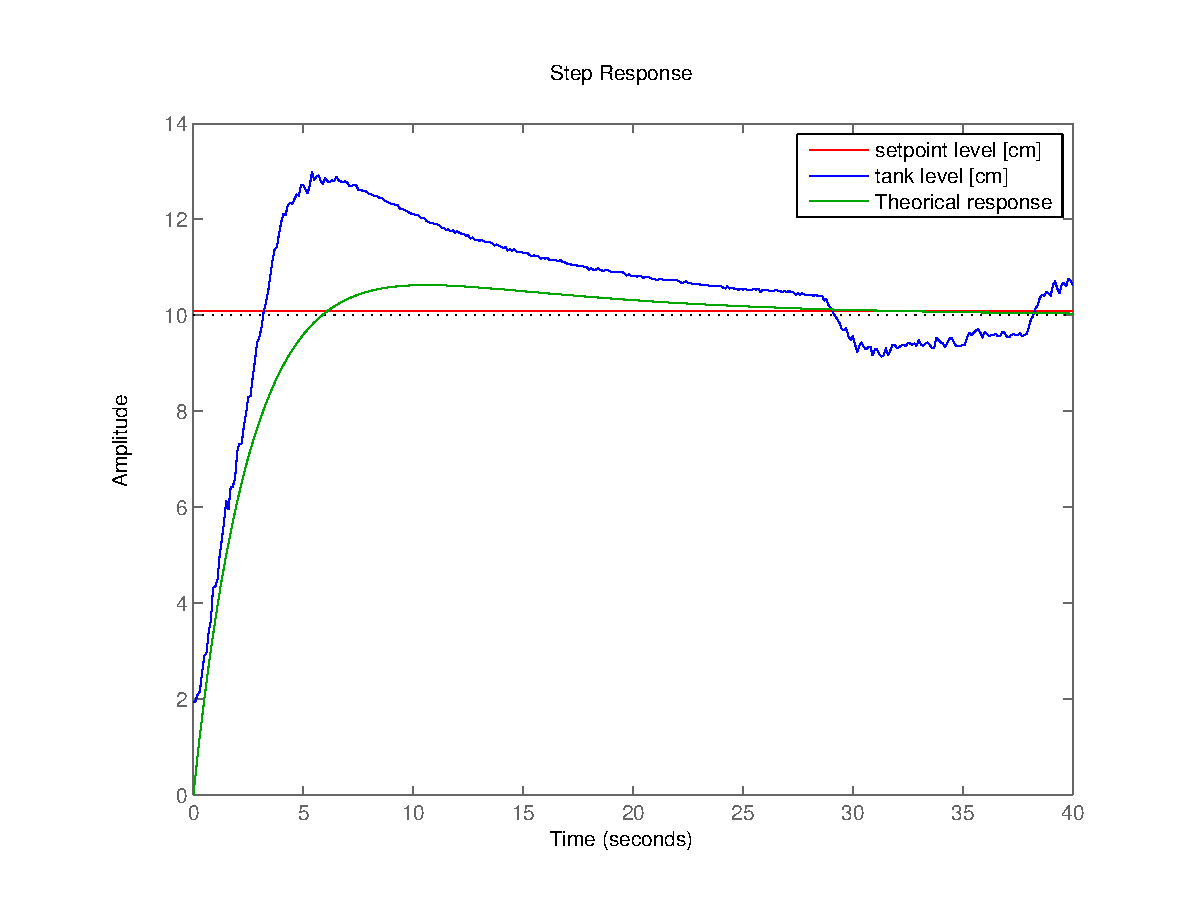
\includegraphics[width=0.8\linewidth]{img/cl_ultimate_without_simplification.eps}
	\caption{Réponse du système avec $\left\{K_P,K_I \right \} = \left\{18.97,0.089\right\}$.}
	\label{fig:final_values_1}
\end{figure}

\subsection{Avec simplification pôle-zéro}
En posant 
\begin{equation}
	K_I = -A
\end{equation}
on obtient une simplification pôle-zéro, et la fonction de transfert devient
\begin{equation}
	T_r(s) = \frac{K_P B_u}{s+K_P B_u}= \frac{1}{1+\frac{s}{K_P B_u}}.
\end{equation}

S'agissant d'une fonction du premier ordre, il n'y a pas de dépassement, et le temps de réponse vaut 
\begin{equation}
	\tau = \frac{1}{K_P B_u} = \frac{\tau_{OL}}{3} 
\end{equation}

On trouve les valeurs chiffrées suivantes
\begin{align}
	K_P &= 4.55\\
	K_I &= 0.035
\end{align}
La comparaison théorie/résultats se trouve à la figure \ref{fig:final_values_2}.

\begin{figure}[!ht]
	\centering
	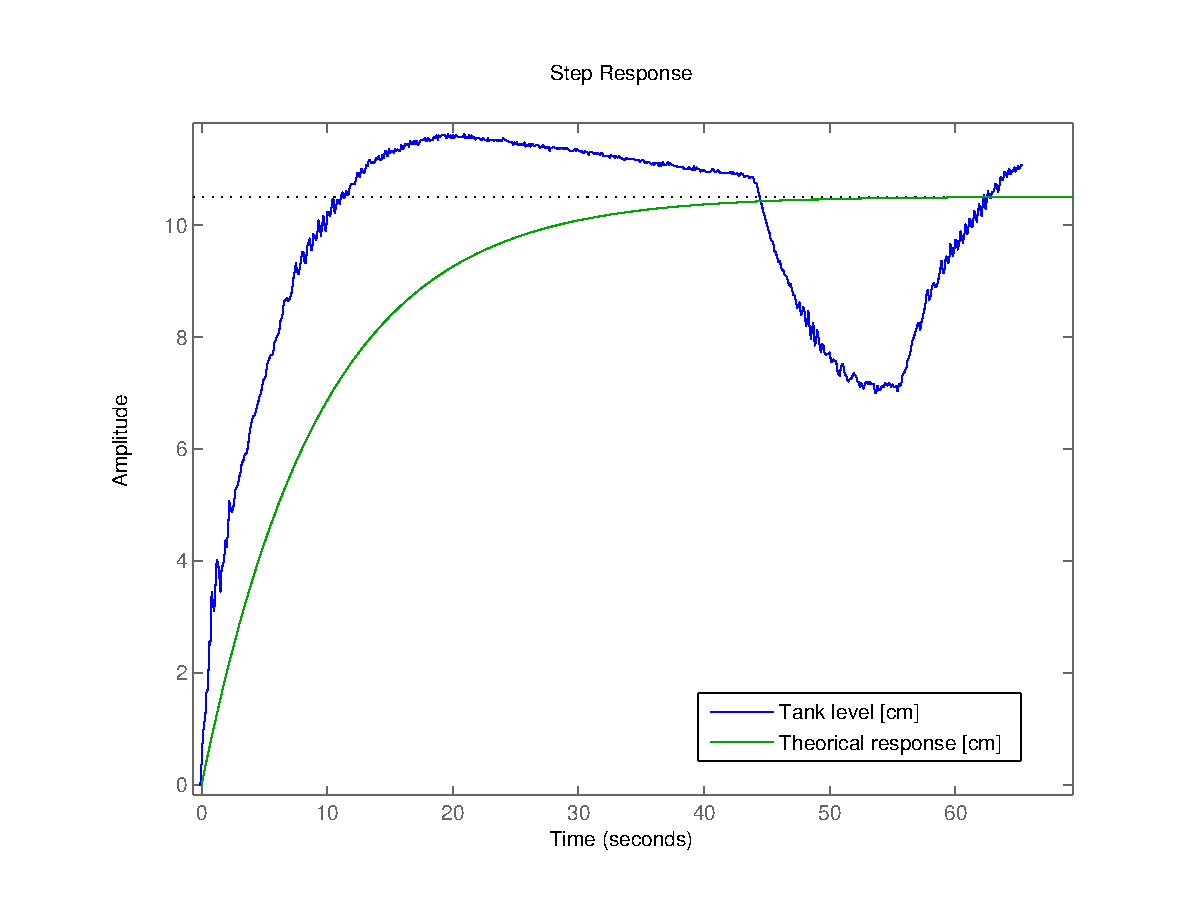
\includegraphics[width=0.8\linewidth]{img/cl_ultimate.eps}
	\caption{Réponse du système avec $\left\{K_P,K_I \right \} = \left\{4.55,0.035\right\}$
	(obtenue avec simplification pôle-zéro.}
	\label{fig:final_values_2}
\end{figure}

\section{Non-linéarités du système contrôlé}
La non-linéarité principale vient du fait que le système d'équations initiales n'est pas linéaire,
et qu'il a dû être linéarisé autour de son point d'équilibre. Ainsi, lorsque l'on ne se trouve
pas proche de ce point d'équilibre, les équations que nous avons ne sont pas correctes.

\end{document}